\begin{samepage}
\chapter{Komponentensemantik}

\subsubsection*{Komponentendiagramm}
... zeigt die austauschbaren Komponenten inkl. ihrer Schnittstellen im System. Es wird zwischen angebotenen und genutzten Schnittstellen unterschieden. Eine Komponente kann dabei aus mehreren Klassen des Klassendiagramms bestehen.
\nopagebreak[4]
\begin{figure}[hbt]
  \centering
  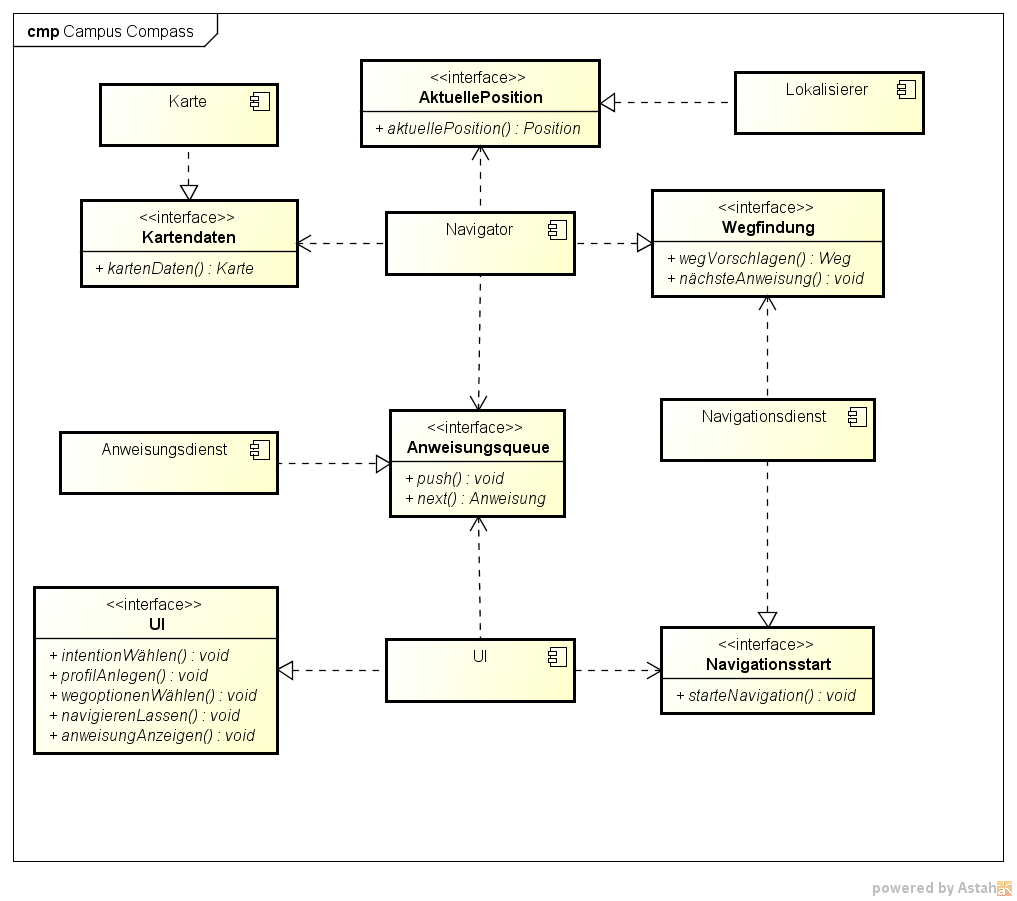
\includegraphics[scale=0.45]{img/komponentendiagramm_neu.png}
  \label{img:komponentendiagramm}
  \caption{Komponentendiagramm}
\end{figure}
\nopagebreak[4]
In der Betrachtung der Systemkomponenten des Campus Compass, sind die modularen Komponenten des Systems zu sehen. Die gezeigten Komponenten werden als modular bezeichnet, da ja dieser Komponenten für sich austauschbar ist.
\nopagebreak[4]
\end{samepage}